\graphicspath{{./chapitres/chapitre1/figures/}}
\setcounter{mtc}{1}
\chapter{\'Présentation du cadre général du projet}
\fancyhead[R]{\ungaramond\small\textbf{Chapitre 1: \'Etude préalables}}
\minitoc
\newpage
%\minilof
\section*{Introduction}
Ce chapitre a pour objectif de définir l’entreprise d’accueil L’Oréal, la présentation du projet, la problématique, l’étude et critique de l’existant. Nous détaillons par la suite les principaux objectifs de ce projet. Pour finir par exposer la méthodologie de travail adoptée pour le réaliser.

\section{Présentation de l'organisme d'accueil}
La figure présente le logo de L’Oréal un groupe industriel français de produits cosmétiques siégé à Clichy, Paris présent dans 130 pays sur les cinq continents. La société, créée par Eugène Schueller le 30 juillet 1909, est aujourd'hui le leader mondial du secteur avec un chiffre d'affaires de 29 milliards d'euros.

\\ Les marques de L'Oréal sont organisées par circuit de distribution selon 4 divisions : les produits professionnels, les produits grand public, L'Oréal Luxe et la cosmétique active. Les marques sont de toutes les origines culturelles : Européennes, Américaines, Chinoises, Japonaises, Coréennes, Brésiliennes, Indiennes et Africaines. [1]

\begin{figure}[!ht]\centering
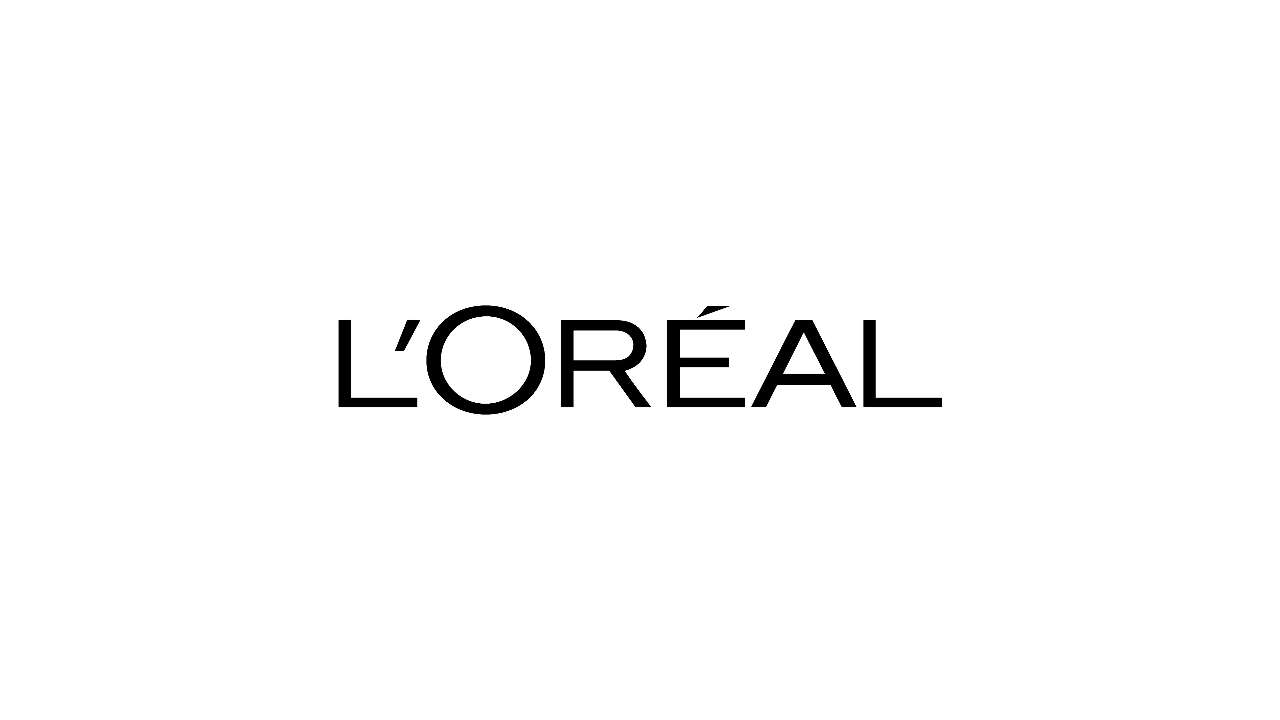
\includegraphics[width=0.4\textwidth]{chapitres/chapitre1/figures/big.jpeg}
\caption{Le\textcolor{white}{J}logo\textcolor{white}{J}de\textcolor{white}{J}l'organisme}
\label{fig:equalioslogo}
\end{figure}

\section{Presentation du sujet}
L’impact du digital sur le marché de la beauté semble être largement partagé. En se digitalisant, les entreprises gagnent du temps, de l’espace et de l’argent. La digitalisation bénéficie indéniablement de l’innovation, car elle permet d’être de plus en plus compétitif au moindre coût. 
L’Oréal investit massivement dans l’intelligence artificielle, la réalité augmentée, le développement d’applications afin d’améliorer son positionnement et être pionnière dans la "Beauty Tech".
Pour cela, L’Oréal m’a engagé pour concevoir, développer et mettre en œuvre un nouveau processus de développement de nuances de couleur de cheveux et la réduction du Time To Market des produits de coloration de cheveux de manière substantielle.

\newpage
\section{Problématique}
La coloration des cheveux était la première activité lancée par L’Oréal. La marque a mis sur le marché une large gamme de produits de coloration : colorants permanents, semi-permanents et même une coloration permanente translucide. La qualité de ces teintures capillaires est sans précédent et les produits sont donc utilisés dans les salons du monde entier avec 1,5 million de coiffeurs et 350 000 salons partenaires.
Pour maintenir son positionnement de leader mondial, L’Oréal a toujours veillé à développer ses processus de production et notamment le processus d’alignement entre le département de la chimie responsable de la composition des formules des teintes de cheveux et le département marketing appelé à répondre au besoin du marché qui mérite d’être continuellement optimisé.

\section{Étude de l’existant}
Le processus de coordination entre le département chimie et le département marketing est totalement manuel. 
Après des séances de travail et d’échange entre le chimiste et le marketteur pour le choix des teintes de cheveux à préparer, le chimiste procède à la préparation des teintes de cheveux convenues et les présente au marketteur pour validation.
Ce processus de validation, relativement lent, prend en moyenne trois mois pour une validation finale des teintes à produire. 

\section{Critique de l’existant}
Comme indiqué précédemment, le processus de coordination entre le département chimie et le département marketing est relativement lent et totalement manuel.
Il ne permet pas un développement soutenu des teintes de couleur et leur traçabilité d’une part et une réponse rapide aux besoins du marché d’autre part.

\section{Solution proposée}
Face aux limites du processus de coordination actuel, la solution proposée consiste à digitaliser ce processus en développant une application permettant un alignement entre les deux départements suscités. Cette application va permettre de développer, d’une manière importante, les teintes de cheveux et leurs traçabilités et de réduire le temps de validation des teintes et par conséquent le délai de commercialisation.
L’objectif du projet consiste à réduire le temps d’itération entre le chimiste et le marketeur de 3 mois à 3 semaines environ.

\section{Méthodologie de développement}
Un projet professionnel nécessite un travail bien ordonné qui respect les deadlines alloués à chaque tâche du projet. Une méthodologie bien spécifiée est requise pour aboutir à cette démarche et mènera le projet à terme. 

\subsection{Comparaison et choix de la méthodologie}

\begin{table}[h!]
\center
\begin{tabular}[b]{|m{5cm}|m{5cm}|m{5cm}|}
\hline
\rowcolor{white}
 & Méthodologies lourdes  & Méthodologies agiles \\
\hline
Cycle de vie & En cascade ou en V , sans rétroaction possible & Itérative et incrémentale \\
\hline
Planification & Basée sur la prédiction & Basée sur l’adaptation \\
\hline
Équipe & Interaction entre les membres de l’équipe afin de prendre les décisions et se diviser les tâches & Interaction entre les membres de l’équipe afin de prendre les décisions et se diviser les tâches \\
\hline
Changement & Pas possible & Possible \\
\hline
Qualité & Le client visualise le projet en fin de cycle & Le client visualise le projet au fur et mesure de son exécution \\
\hline
\end{tabular}
\caption{Tableau comparatif des méthodologies lourdes et agiles}
\textcolor{white}{I} \label{tab:tab-m}
\end{table}


Suite à la comparaison entre les deux méthodes dans le tableau \ref{tab:tab-m}, on a opté pour la méthode agile pour plusieurs raisons notamment : 
- Une bonne communication entre le client et l’équipe du projet ce qui favorise un lien de confiance entre eux. 
- Une visibilité par le client sur le projet au fur et à mesure de son exécution. 
-Une flexibilité au changement lors du développement du projet. 
- Un contrôle qualité au fil de l’eau.

\subsection{Scrum}
Afin d’aboutir à l’exécution de ce projet, la méthodologie agile Scrum choisie est la méthode agile la plus connue et la plus utilisée qui assure une bonne communication entre les membres de l’équipe et favorise le bon déroulement de chaque projet tout en permettant au client une bonne visibilité tout au long de l’exécution.
 Le travail est divisé en Sprints, chaque sprint dure entre 1 à 4 semaines selon sa difficulté et complexité. La figure présente le processus de SCRUM, les membres de l’équipe et les documents qui seront générés.
\begin{figure}[!ht]\centering
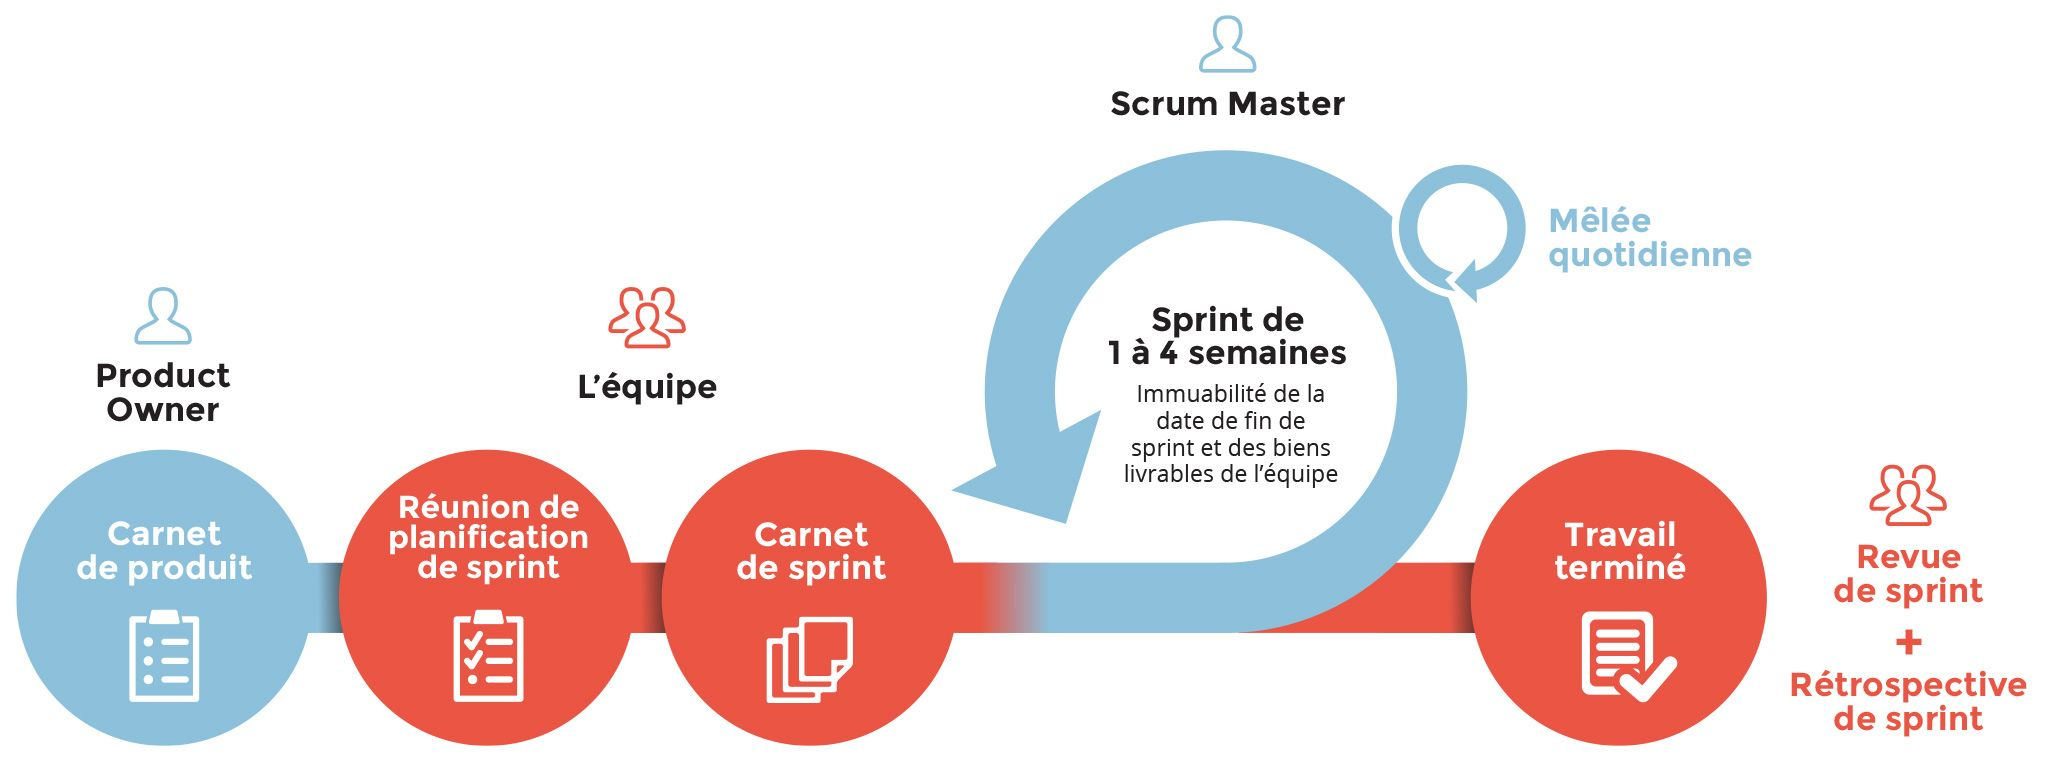
\includegraphics[width=0.8\textwidth]{chapitres/chapitre2/figures/scrum.jpeg}
\caption{Principe\textcolor{white}{J}de\textcolor{white}{J}la\textcolor{white}{J}méthodologie\textcolor{white}{J}Scrum}
\label{fig:fig2}
\end{figure}

\newpage
\paragraph{Product\textcolor{white}{I} Owner} 
C’est celui qui se charge de transmettre la vision du client sur le produit qu’il souhaite avoir tout en détaillant ses besoins fonctionnels, c’est lui donc qui rédige le Backlog produit.

\paragraph{Scrum\textcolor{white}{I} Master}
C’est un motivateur d’équipe et un coach agile, sa tâche principale est l’assurance de la bonne entente et cohésion entre les membres de son équipe, il garantit ainsi la bonne application de la méthode SCRUM.


\paragraph{Scrum\textcolor{white}{I} Team}
Ce sont des individus polyvalents de différents secteurs, supervisés par leur SCRUM master ainsi que le Product Owner. Ils ont pour mission principale l’élaboration des différents sprints demandés.


\section*{Conclusion}
Dans le premier chapitre, nous avons mis en place le sujet dans le cadre général en commençant par une présentation de l’entreprise et du projet, en passant par la problématique ensuite par faire l’étude de l’existant et sa critique, nous avons abouti par la suite à la solution proposée et nous avons fini ce chapitre par choisir la méthode de travail.
